% !TEX program = xelatex
% Compile: xelatex poster.tex   (A1 landscape academic poster, `make poster`)
\documentclass[final]{beamer}
\usepackage[scale=1.15, size=a1, orientation=landscape]{beamerposter}
\usepackage{ctex}
\usepackage{graphicx}
\usepackage{booktabs}
\usepackage{tikz}
\usetikzlibrary{positioning, arrows.meta, calc, fit}
\usepackage[most]{tcolorbox}

% ---- palette ----
\definecolor{urcyan}{RGB}{6, 182, 212}
\definecolor{urink}{RGB}{30, 41, 59}
\definecolor{urbody}{RGB}{248, 250, 252}
\definecolor{uramber}{RGB}{240, 178, 64}
\definecolor{urgreen}{RGB}{34, 197, 94}
\definecolor{urgrid}{RGB}{226, 232, 240}

\setbeamertemplate{navigation symbols}{}
\setbeamercolor{background canvas}{bg=white}
\setbeamercolor{block title}{bg=urink, fg=white}
\setbeamercolor{block body}{bg=urbody, fg=urink}
\setbeamerfont{block title}{size=\large, series=\bfseries}
\setbeamerfont{block body}{size=\normalsize}
\setbeamertemplate{blocks}[rounded][shadow=false]
\setbeamertemplate{itemize items}[circle]
\setbeamercolor{itemize item}{fg=urcyan}
\setbeamercolor{itemize subitem}{fg=urcyan}

\begin{document}
\begin{frame}[t]{}

% ============================================================ Title band
\begin{tcolorbox}[colback=urink, colframe=urink, sharp corners, boxrule=0pt,
   borderline south={4pt}{0pt}{urcyan},
   halign=center, left=20pt, right=20pt, top=20pt, bottom=18pt]
{\color{white}\fontsize{54}{62}\selectfont\bfseries
 基于 Newton 物理引擎与 Claude VLA 的具身智能交互演示}\\[12pt]
{\color{urcyan!40!white}\large
 CPU-only 课堂级具身智能交互系统 \;——\; 经典控制 · 混合 VLA 解析 · 真实物理仿真}
\end{tcolorbox}

\vspace{0.7cm}

% ============================================================ Abstract
\begin{tcolorbox}[colback=urbody, colframe=urgrid, boxrule=1pt, rounded corners,
   left=18pt, right=18pt, top=12pt, bottom=12pt]
{\large\bfseries\color{urink} 摘要\quad}{\normalsize\color{urink}
本工作在一台无 GPU、无云依赖的 MacBook 上实现 3 分钟课堂级具身智能交互演示，集成
NVIDIA Newton XPBD 物理引擎、pygame 二维渲染与 Claude 命令行（作为视觉--语言--动作意图
解析器）。系统提供三种交互：基于闭式弹道反解的接球、自然语言驱动的抓取与堆叠、装饰性手势；
v0.2.0 进一步引入真实刚体方块、双臂协作搭塔与偏移塔稳定性实验。三项核心贡献为
(1) 关键词预飞 + Claude 后台精化的\textbf{混合解析管线}，将命令到动作延迟由约 9.4 s 降至 1 ms；
(2) 无 weld 约束的 XPBD 上以 \textbf{KINEMATIC$\leftrightarrow$DYNAMIC 翻转}实现夹爪抓取；
(3) 将物理步进开销由 11.9 ms 降至 0.30 ms 的\textbf{三级优化}。系统经 250 项单元与集成测试覆盖。}
\end{tcolorbox}

\vspace{0.7cm}

% ============================================================ 3 columns
\begin{columns}[t]

% -------------------------------------------------- Column 1
\begin{column}{0.315\linewidth}

\begin{block}{1\;\; 引言与动机}
\normalsize
大语言模型已能写代码、规划、对话，但``身体''仍是其缺失的一环。课堂场景中，学生难以直观
区分\textbf{经典控制}与\textbf{学习驱动}，亦难以亲手验证大模型在闭环物理中的行为。本系统
将二者并置于同一可交互画面，降低具身智能教学的硬件与认知门槛。
\end{block}

\vspace{0.55cm}

\begin{block}{2\;\; 三种交互模式}
\normalsize
\begin{itemize}\setlength\itemsep{7pt}
  \item \textbf{接球}——单步闭式弹道反解（经典控制，无 AI）。固定种子自动基准命中 92--100\%。
  \item \textbf{自然语言驱动}——Claude 解析模糊语义为结构化动作。定位为
        \textbf{LLM 意图解析器}（L$\to$A），区别于 RT-2 式端到端 VLA（无像素输入）。
  \item \textbf{装饰手势}——wave / point / bow / dance。
\end{itemize}
\end{block}

\vspace{0.55cm}

\begin{block}{3\;\; 接球控制与推理可视化}
\centering
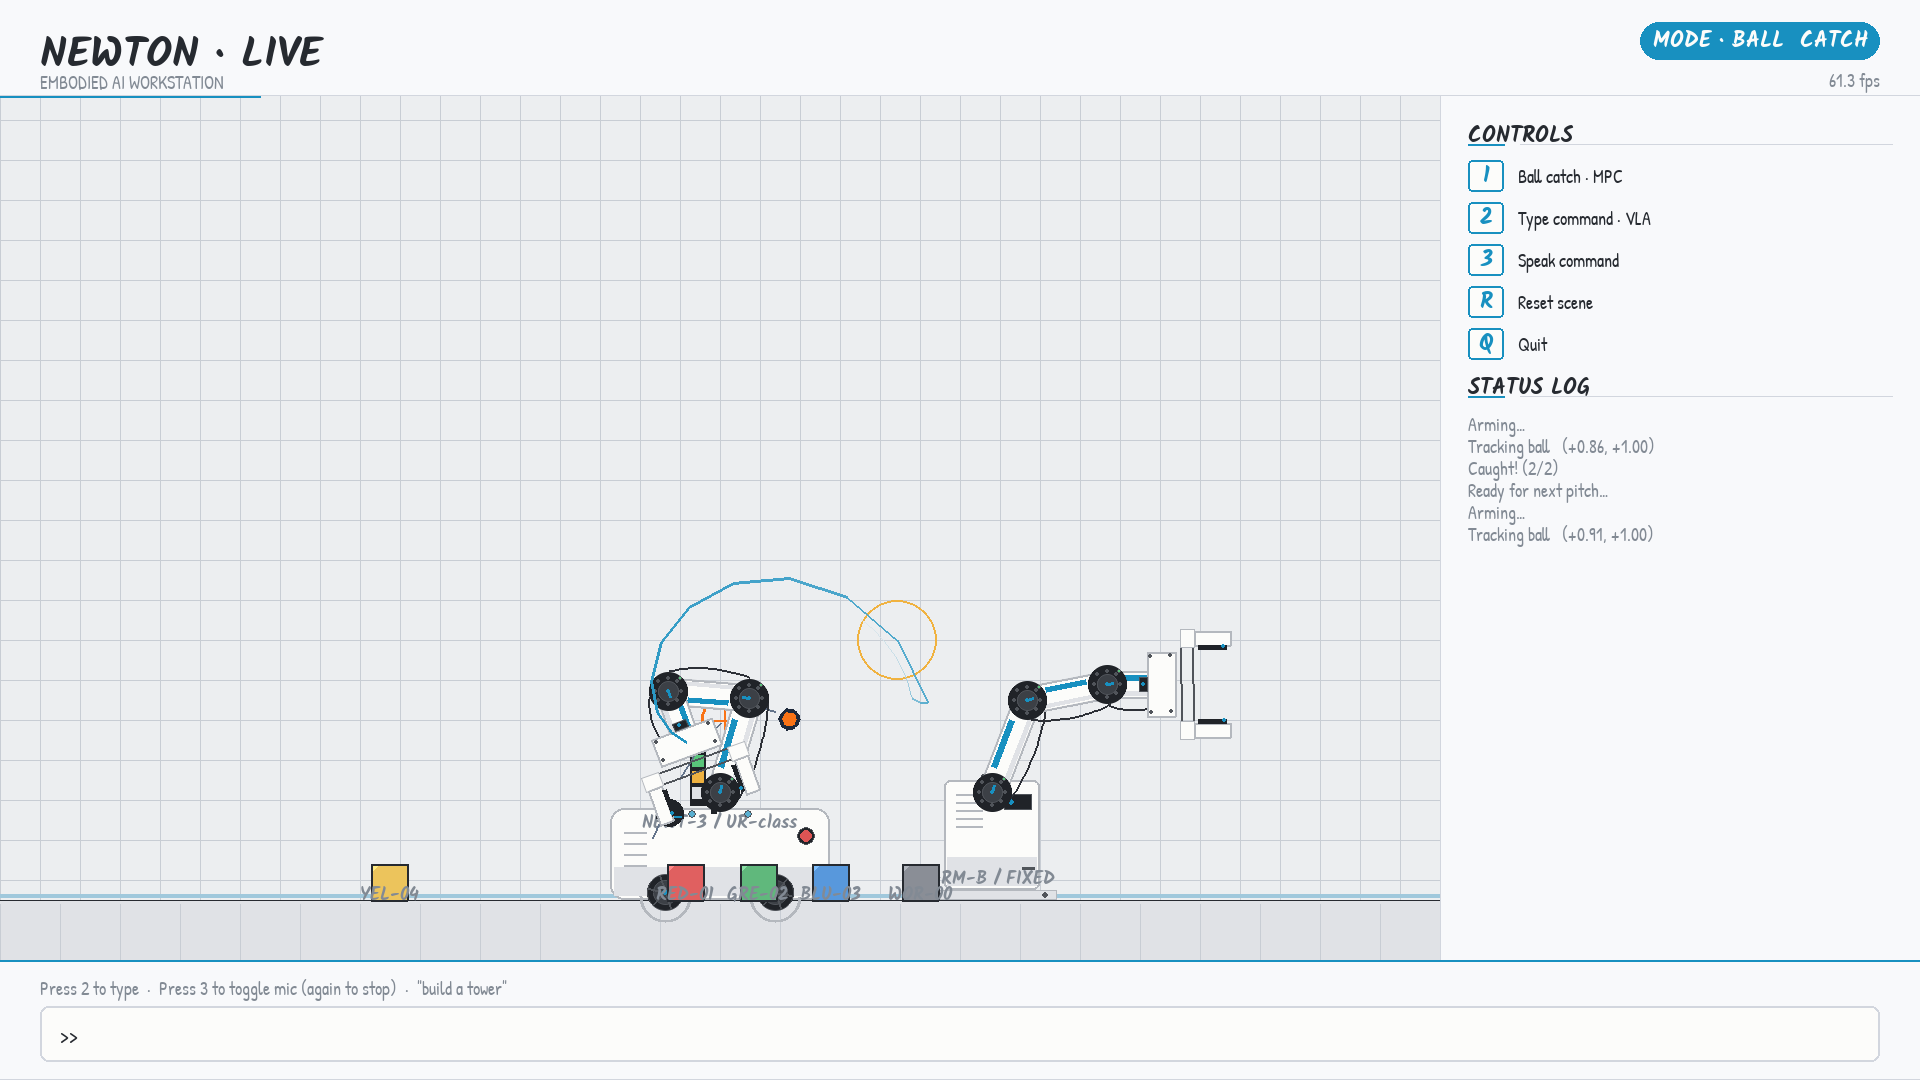
\includegraphics[width=\linewidth]{figures/catch_industrial.png}\\[3pt]
{\footnotesize 蓝色轨迹采样 + 橙色截击圆环；每帧 1 ms 内闭式解算，零优化器。}\\[8pt]

\includegraphics[width=\linewidth]{figures/vla_panel_industrial.png}\\[3pt]
{\footnotesize AI · PARSED 侧栏逐字段展示原话、后端、延迟与解析动作，使解析过程可解释。}
\end{block}

\end{column}

% -------------------------------------------------- Column 2
\begin{column}{0.315\linewidth}

\begin{block}{4\;\; 系统架构}
\normalsize
五层单向数据流：\textbf{输入} $\to$ \textbf{解析}（vla / voice / pipeline）$\to$
\textbf{控制}（tasks / control / catcher）$\to$ \textbf{物理}（Newton XPBD）$\to$
\textbf{渲染}（scene / effects）；telemetry 横切各层并写 CSV。共 22 模块、约 7730 行。
关注点分离使解析层可替换大模型而不影响下游控制与物理。
\end{block}

\vspace{0.55cm}

\begin{block}{5\;\; 方法：混合 VLA 解析管线}
\normalsize
Claude 端到端延迟 2--10 s，远超 60 fps 帧预算。本方法\textbf{解耦行动与推理}：
\begin{itemize}\setlength\itemsep{5pt}
  \item 关键词预飞 $\sim$1 ms 同步派单，机械臂即时启动；
  \item Claude 后台线程 $\sim$9.4 s 返回，与预飞结果比较确认；
  \item generation counter 防止过期线程覆盖新命令。
\end{itemize}
\vspace{3pt}
\centering
\begin{tikzpicture}[font=\small]
  \draw[-Stealth, very thick, gray] (0,0) -- (19,0) node[right]{$t$};
  \node[fill=urgreen!80!black, rounded corners=3pt, minimum width=0.5cm, minimum height=0.7cm] at (0.35,1.5){};
  \node[right, urgreen!45!black] at (0.9,1.5){\textbf{1 ms} 预飞 $\to$ 臂动};
  \node[fill=uramber, rounded corners=3pt, minimum width=9.5cm, minimum height=0.7cm, anchor=west] at (0,0.55){};
  \node[white] at (4.7,0.55){Claude 后台分析 $\sim$9.4 s};
\end{tikzpicture}\\[2pt]
{\footnotesize 命令到动作的感知延迟由 9.4 s 降至 1 ms（该 1 ms 来自预飞，而非 Claude）。}
\end{block}

\vspace{0.55cm}

\begin{block}{6\;\; 演示流程（连续运行实录）}
\centering
\setlength{\tabcolsep}{4pt}\renewcommand{\arraystretch}{0.9}
\begin{tabular}{cc}
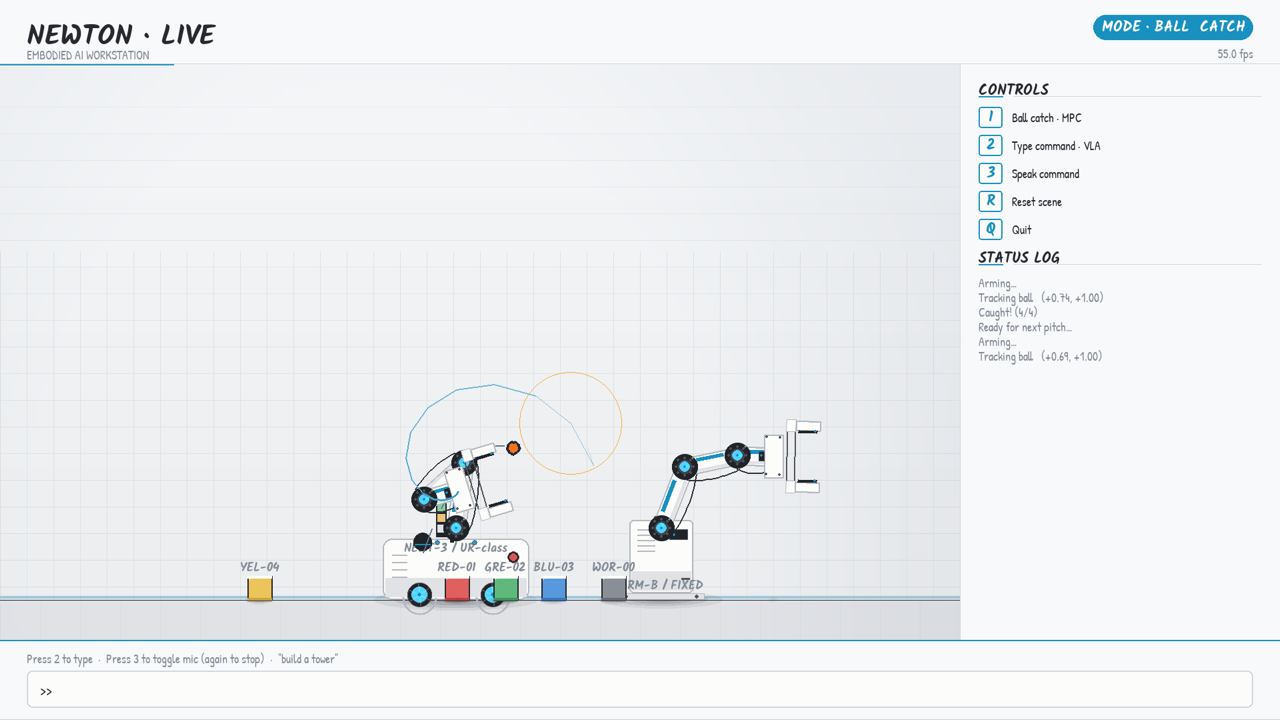
\includegraphics[width=0.47\linewidth]{figures/flow_1_catch.png} &
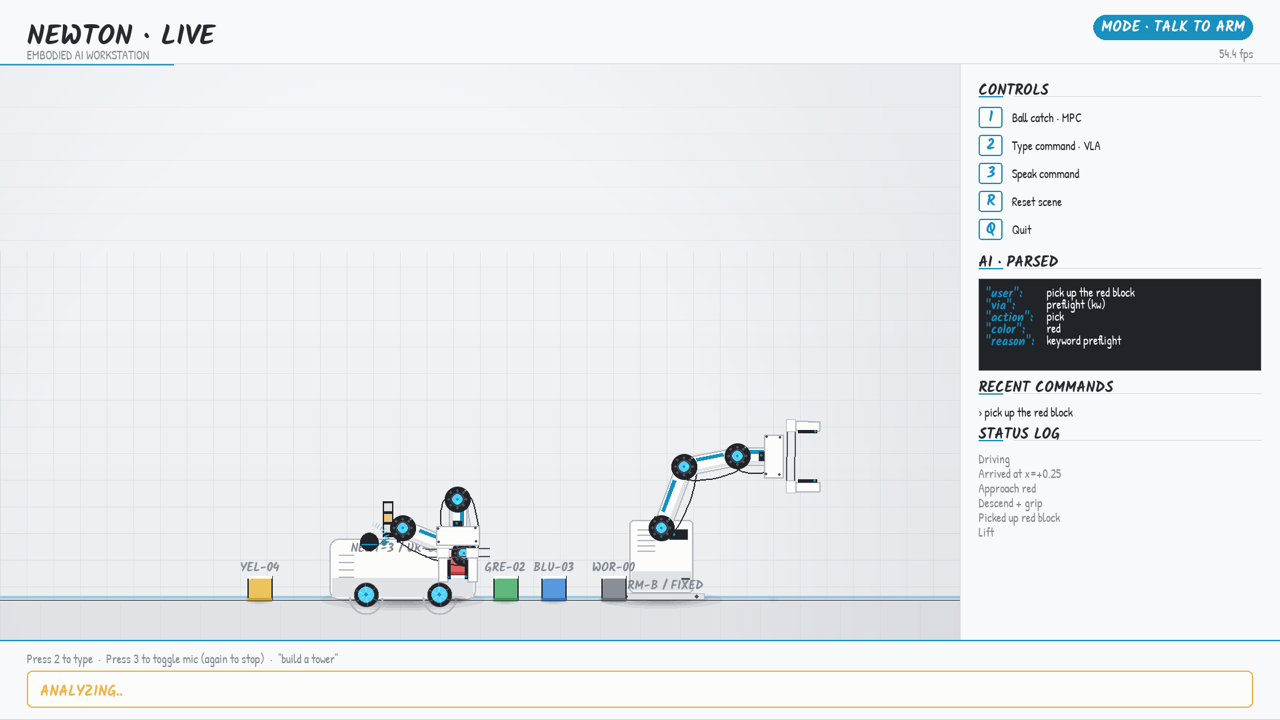
\includegraphics[width=0.47\linewidth]{figures/flow_2_typed.png}\\
{\footnotesize 1) 接球 MPC} & {\footnotesize 2) 打字：预飞派单 + 后台}\\
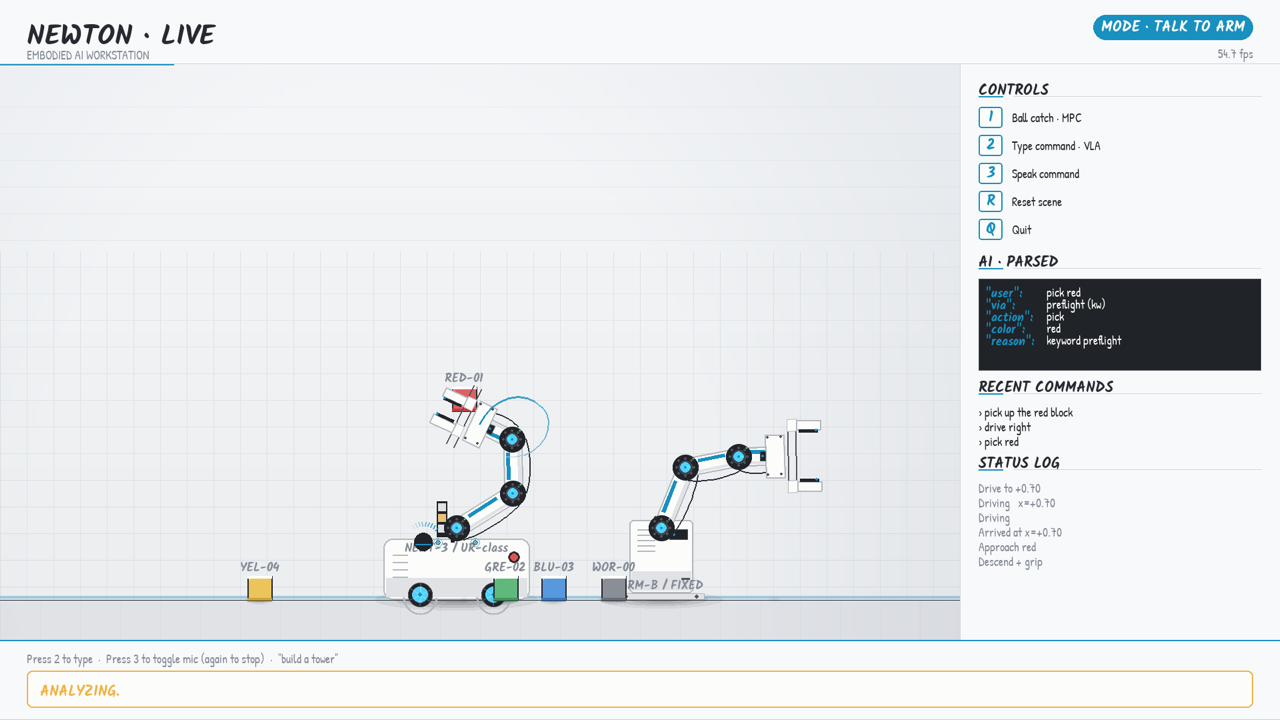
\includegraphics[width=0.47\linewidth]{figures/flow_3_voice.png} &
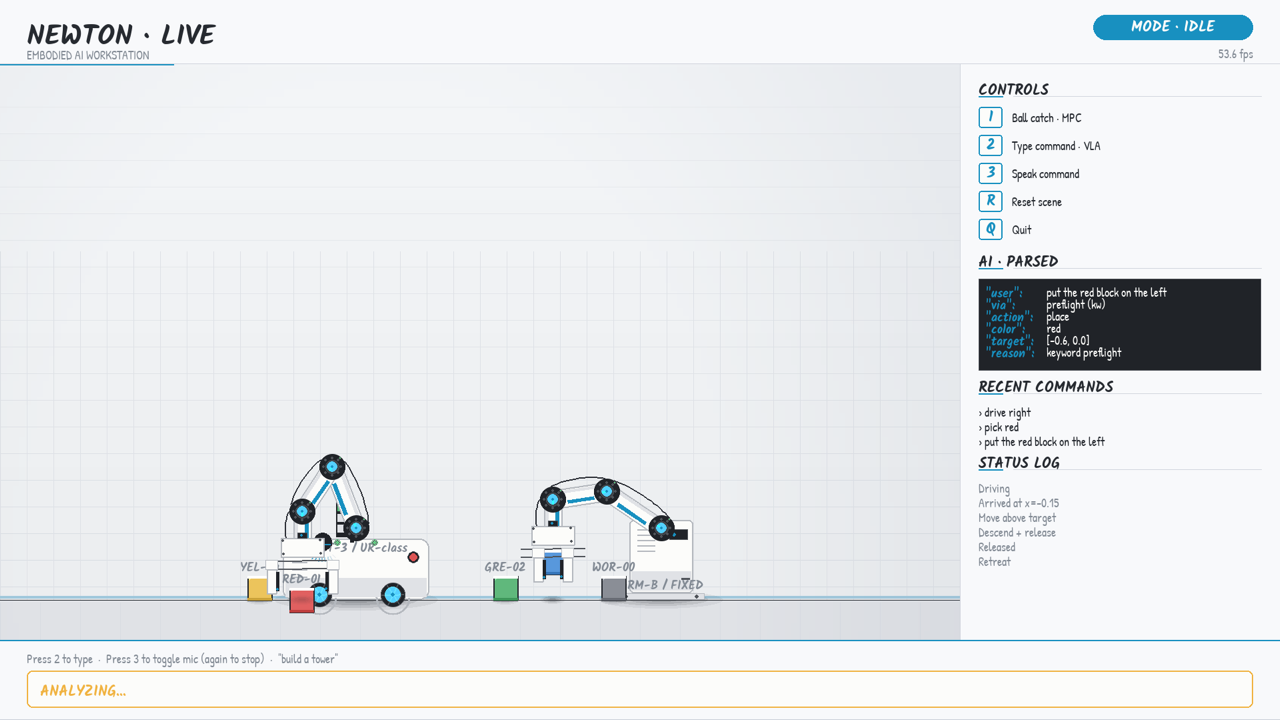
\includegraphics[width=0.47\linewidth]{figures/flow_4_dual.png}\\
{\footnotesize 3) 语音模糊匹配} & {\footnotesize 4) 双臂并行}\\
\end{tabular}\\[2pt]
{\footnotesize 阶段 2) 中预飞派单、机械臂已抓取时 Claude 仍在分析，体现管线的延迟解耦。}
\end{block}

\end{column}

% -------------------------------------------------- Column 3
\begin{column}{0.315\linewidth}

\begin{block}{7\;\; v0.2.0：真实物理与协作}
\normalsize
\begin{itemize}\setlength\itemsep{5pt}
  \item \texttt{--real-blocks}：方块为真实 Newton 刚体。XPBD 无 weld 约束，抓取以
        \textbf{KINEMATIC$\leftrightarrow$DYNAMIC} 翻转实现。
  \item \texttt{--collab}：双臂接力搭塔，单交接槽互锁 + 时序不对称避免冲突。
  \item \texttt{--experiment}：偏移塔稳定性物理实验（见下）。
\end{itemize}
\end{block}

\vspace{0.55cm}

\begin{block}{8\;\; 实验结果：偏移塔稳定性（理论 vs 仿真）}
\centering
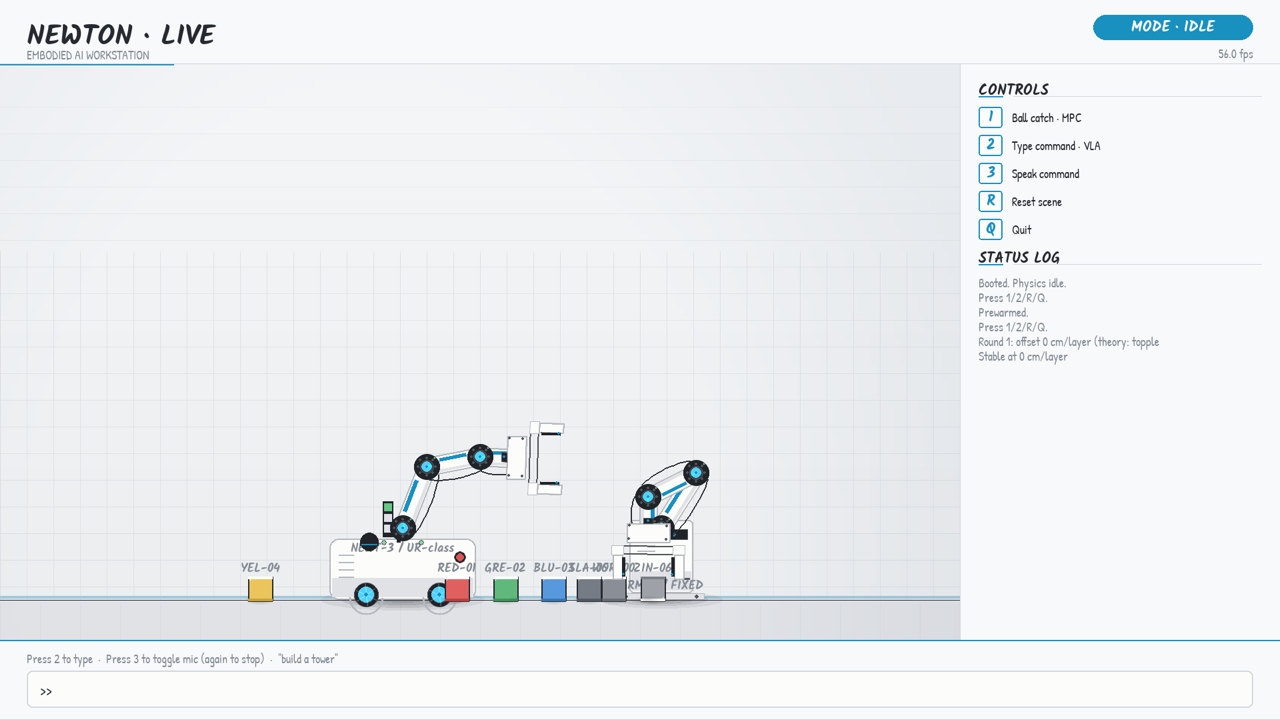
\includegraphics[width=0.32\linewidth]{figures/experiment_aligned.png}\hfill
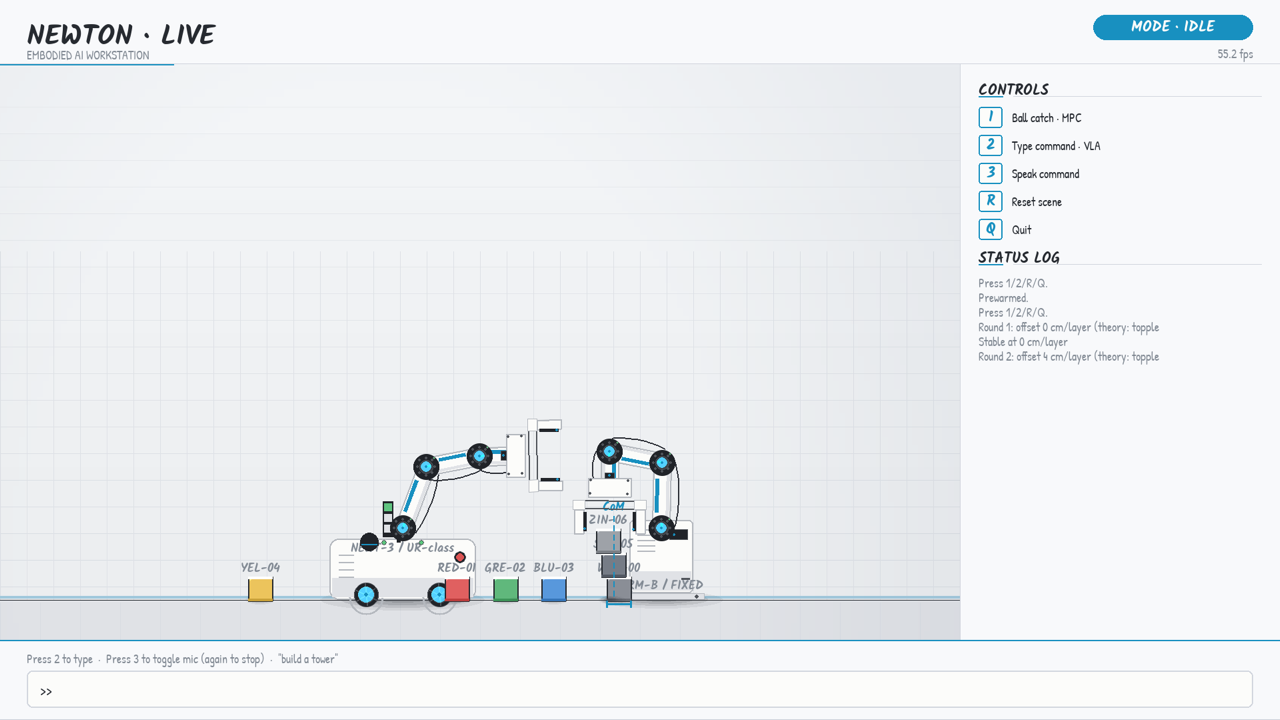
\includegraphics[width=0.32\linewidth]{figures/experiment_offset.png}\hfill
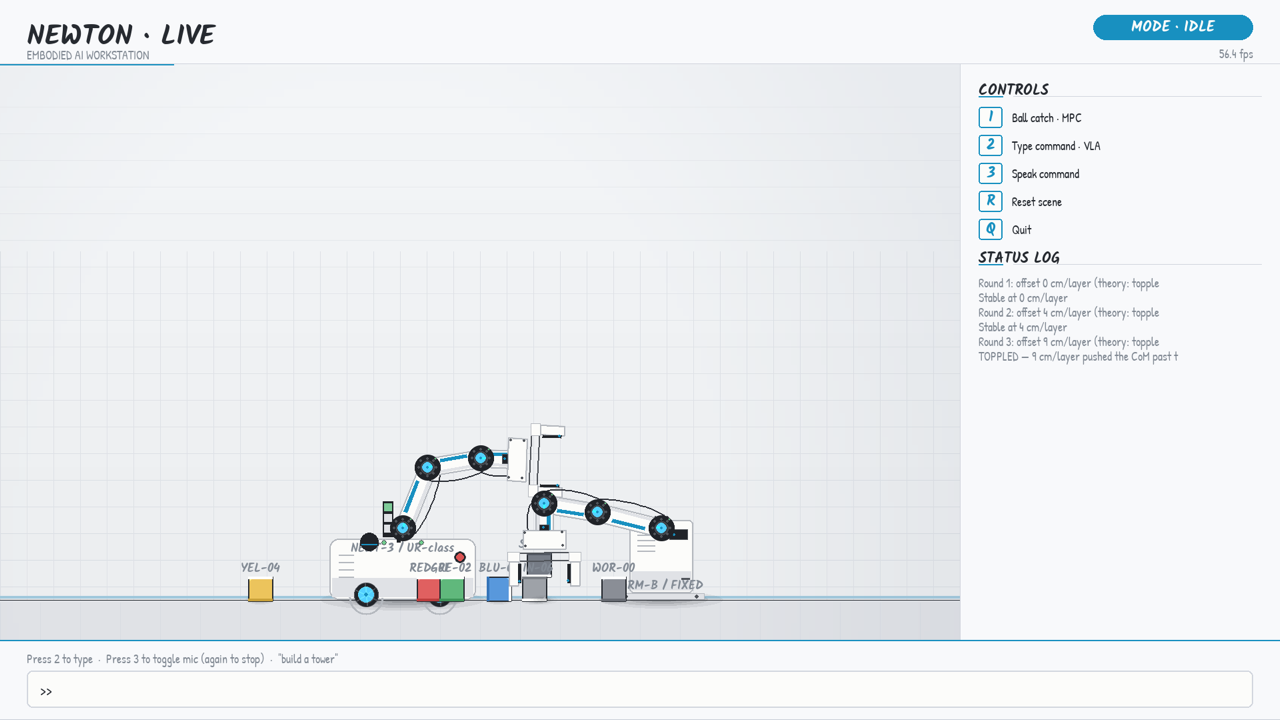
\includegraphics[width=0.32\linewidth]{figures/experiment_topple.png}\\[3pt]
{\footnotesize 逐层偏移 0 / 4 / 9 cm：稳 · 稳 · 倒（重心铅垂线越界变色）}\\[6pt]
\normalsize 刚体理想判据 $1.5d>r\Rightarrow d>6.67$ cm；真实 XPBD 实测倒塌边界落在
$(4,5]$ cm（接触柔度使其更早失稳）。所选 0 / 4 / 9 三档的稳/倒判定与理论同号，
倒塌由求解器判定而非脚本设定。
\end{block}

\vspace{0.55cm}

\begin{block}{9\;\; 性能评估}
\normalsize
\texttt{world.step()} 原占 11.9 ms（71\% 帧预算），其主体为 Warp 内核\textbf{启动开销}
而非计算。经降迭代/子步与 teleport 跳过碰撞等优化降至 \textbf{0.30 ms（约 40$\times$）}，
uncapped 吞吐由 64 升至 \textbf{279 fps}。渲染臂由控制器前向运动学驱动，降迭代对画面无影响。
\end{block}

\vspace{0.55cm}

\begin{block}{10\;\; 评估与结论}
\normalsize
250 项单元与集成测试（100\% 通过），偏移塔倒塌边界由真求解器回归测试固定。系统在无 GPU、
无云的消费级硬件上实现了可解释、低延迟、可复现的具身智能教学演示。\par
\vspace{5pt}
{\footnotesize\color{urink!70}
项目主页\;\texttt{hollis36.github.io/newton-vla-demo} \quad·\quad
源码\;\texttt{github.com/Hollis36/newton-vla-demo}（MIT, v0.2.0）}
\end{block}

\end{column}
\end{columns}

\end{frame}
\end{document}
